\documentclass[oneside, master=eelt,masteroption=ec]{kulemt}
\setup{
  title={Detecting Cyber Threats with Machine Learning: A Comparative Analysis of Linear, Tree-Based, and Neural Models },
  author={Marti Geudens \and r0934872 \and Piet Verguts \and r0954535},
  promotor={Prof.\,dr.\,ir.\ Knows Better},
  assessor={Ir.\,Kn. Owsmuch\and K. Nowsrest},
  assistant={Diwas Lamsal}}
% Remove the "%" on the next line for generating the cover page
%\setup{coverpageonly}
% Remove the "%" before the next "\setup" to generate only the first pages
% (e.g., if you are a Word user).
%\setup{frontpagesonly}

% If you want to include other LaTeX packages, do it here. 

% Finally the hyperref package is used for pdf files.
% This can be commented out for printed versions.

\usepackage[table]{xcolor} % 'table'optie is handig voor cell backgrounds
\usepackage{xltabular}    % combinatie van longtable + tabularx
\usepackage[table]{xcolor}
\usepackage{enumitem}
\usepackage{xltabular,enumitem} 
\usepackage[table]{xcolor} 
\usepackage{pdflscape}
\usepackage{placeins}
\usepackage{longtable}
\usepackage[pdfusetitle,colorlinks,plainpages=false]{hyperref}
%%%%%%%
%\includeonly{chapter-n}
\begin{document}

\tableofcontents*

\begin{abstract}
  This study evaluates the effectiveness of three distinct machine learning model families, 
  Logistic Regression, Random Forest, and Neural Networks for network intrusion detection 
  using the NSL-KDD benchmark dataset. Motivated by the increasing complexity of cyber threats 
  and recent high-profile breaches, the research compares linear, ensemble-based, 
  and non-linear approaches in both binary and multi-class classification scenarios. 
  Utilizing a unified preprocessing pipeline and addressing severe class imbalance through 
  class-weighted learning and decision-threshold optimization, the project analyzes model performance 
  beyond aggregate accuracy, with a specific focus on rare attack categories like 
  User-to-Root (U2R) and Remote-to-Local (R2L). Key results indicate that while all 
  models achieve high binary accuracy (up to 77.8\%), their ability to generalize to 
  unseen attack patterns in the test set varies significantly. Random Forest provides the 
  best stability and ranking performance (ROC-AUC of 0.962), yet the Neural Network offers 
  superior sensitivity to critical minority attacks, achieving a U2R recall of 0.70. 
  However, the substantial performance drop between validation and test sets highlights 
  that model expressiveness alone cannot overcome the inherent limitations of imbalanced 
  training data. We conclude that while Random Forest offers the most practical balance 
  for general detection, robust multi-class intrusion detection requires data-centric 
  strategies like hierarchical pipelines and anomaly-aware learning to effectively 
  identify rare, high-risk security threats.

\end{abstract}

% If there are only a few figures and tables, it is better to use the following:
\listoffiguresandtables


% Now comes the main text
\mainmatter

\chapter{Introduction}
\label{cha:intro}

In today’s interconnected world, traditional rule-based Intrusion Detection Systems (IDS) struggle to keep pace with the rapid evolution of cyber threats. Attackers continuously adapt their methods by exploiting trust relationships, user behaviour, and system misconfigurations, rendering static detection techniques increasingly ineffective. Machine Learning (ML) has therefore been widely proposed as a suitable approach to address these challenges, and numerous benchmark studies demonstrate its effectiveness in this domain. For example, Abrar et al. show, using the well-known NSL-KDD dataset, that classifiers such as Random Forest (RF), Extra Tree, Decision Tree, and Support Vector Machines (SVM) can achieve very high detection accuracy for classifying normal versus malicious traffic, often exceeding 99\% \cite{abrar2020machine}. Furthermore, Gawand and Meesala confirm that NSL-KDD remains a useful benchmark for prototyping and comparative evaluation, despite the increasing complexity of real-world network traffic \cite{gawand2025improved}. At the same time, NSL-KDD is a benchmark dataset and does not fully capture the characteristics of production networks. Hence, results obtained on this dataset should therefore be interpreted as comparative and methodological rather than indicative of real-world performance.

The need for adaptive intrusion detection is further reinforced by recent large-scale cyber incidents. In 2025, Ingram Micro suffered a ransomware attack by the SafePay group that resulted in the exfiltration of over 3.5 TB of data through compromised VPN credentials. Similarly, Orange SA was targeted by the Warlock group, while Louis Vuitton (LVMH) experienced a data breach via a third-party CRM vulnerability, exposing customer information across multiple European regions. These incidents share common characteristics, such as third-party security vulnerabilities, credential theft, and social-engineering-based intrusions, which frequently bypass traditional IDS solutions. This highlights the practical relevance of ML-based intrusion detection for both research and real-world deployment\cite{pkware2024breaches}.

In this project, intrusion detection is formulated as a supervised classification task using the NSL-KDD dataset, in which preprocessed network connection records are provided as input to machine-learning models that predict whether network traffic is normal or malicious and, in extended experiments, identify the corresponding attack category (i.e. multi-class classification), including Denial of Service (DoS), Probe, Remote-to-Local (R2L), and User-to-Root (U2R) attacks. This work builds upon prior research that has extensively evaluated ML techniques on NSL-KDD. Tavallaee et al. introduced NSL-KDD as a cleaned and rebalanced alternative to the original KDD Cup ’99 dataset, addressing issues such as redundant records and biased attack distributions that previously led to inflated performance estimates \cite{tavallaee2009detailed}. Subsequent studies consistently report that tree-based ensemble models outperform many alternatives due to their ability to capture nonlinear feature interactions and handle class imbalance effectively \cite{abrar2020machine, hegde2024intrusion, hong2021machine}. Other authors have shown that, while deep learning models can achieve strong performance, classical machine-learning methods such as Random Forest often match or exceed their results while offering lower computational cost and greater interpretability \cite{ali2025deep}.

Guided by these findings, this project evaluates multiple machine-learning models for intrusion detection on NSL-KDD, starting with Logistic Regression as a linear baseline, followed by a Random Forest classifier and finally a neural network to assess whether increased model expressiveness could yield additional benefits. By systematically comparing these approaches, the project aims to provide both empirical insight and practical guidance on the suitability of different ML techniques for network intrusion detection.
\chapter{Methods}
\label{cha:1}

\section{Dataset and Features}
This project uses the NSL-KDD dataset, a publicly available benchmark dataset for intrusion detection research \cite{tavallaee2009detailed}. NSL-KDD was introduced by Tavallaee et al. as a cleaned and improved version of the original KDD Cup 1999 dataset, addressing major shortcomings such as redundant records and biased attack distributions that previously led to overly optimistic detection results. The dataset is freely accessible via Kaggle and is widely used for evaluating and comparing machine-learning-based intrusion detection systems \cite{abrar2020machine}. The purpose of the NSL-KDD dataset is to support supervised classification of network traffic into normal and malicious behavior. Each data instance represents a single network connection and is described by a fixed set of features capturing various aspects of network activity. The classification task can be formulated either as binary classification (normal vs. attack) or as multi-class classification, where attacks are grouped into four main categories: Denial of Service (DoS), Probe, Remote-to-Local (R2L), and User-to-Root (U2R), in addition to the Normal class \cite{hegde2024intrusion}.

The dataset consists of 125,973 samples in the training set (KDDTrain+) and 22,544 samples in the test set (KDDTest+), for a total of five classes. The class distribution is highly imbalanced, with DoS attacks dominating the dataset, while R2L and especially U2R attacks are extremely rare. This imbalance reflects realistic attack distributions but also introduces challenges for model training and evaluation, particularly in the multi-class setting \cite{hong2021machine}. Each network connection is described by 41 features, composed of a mix of numeric, categorical, and binary attributes \cite{tavallaee2009detailed}. These include basic connection features (e.g., duration, protocol type, service, flag), content-based features (e.g., number of failed login attempts, file creation counts), and traffic-based features computed over time windows (e.g., connection counts, error rates, and bytes sent or received) \cite{tavallaee2009detailed}. The raw data is stored in text (.txt) format, with each row corresponding to a single connection record.

Figure \ref{fig:combined_class} illustrates the class distribution of the NSL-KDD dataset for both the training and test splits. Severe class imbalance is evident in both partitions, with Normal and DoS traffic dominating the data, while R2L and U2R attacks occur extremely rarely \cite{tavallaee2009detailed}.


\begin{figure}[htbp]
    \centering
    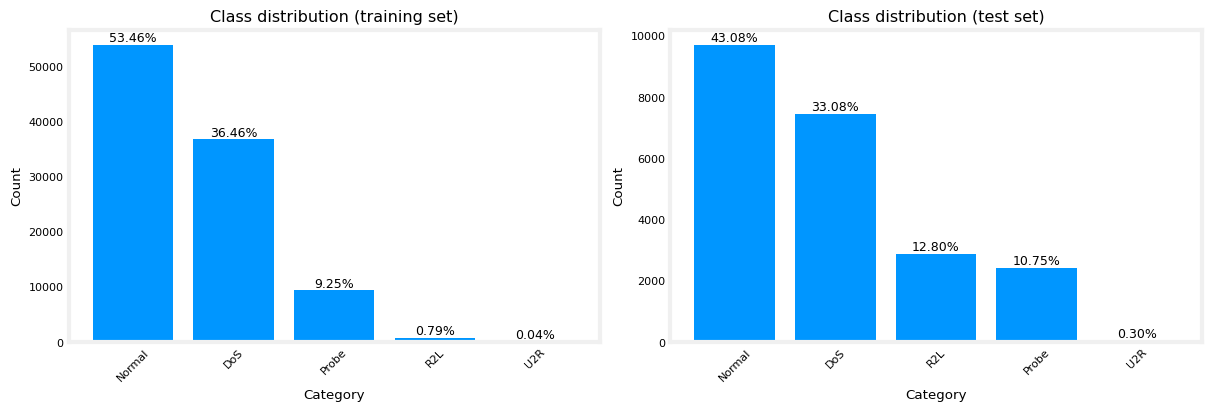
\includegraphics[width=0.9\textwidth]{combined_class.png}
    \caption{Class distribution training vs test}
    \label{fig:combined_class}
\end{figure}

Importantly, the test set exhibits a different class composition than the training set. Although Normal and DoS remain the majority classes, the relative proportions of Probe and R2L attacks increase substantially in the test split. This shift reflects the intentional design of NSL-KDD, in which the test data includes attack types and distributions that are absent or under-represented during training in order to evaluate generalization to previously unseen intrusions \cite{tavallaee2009detailed}. This imbalance and distribution shift have two important implications. First, accuracy alone is a misleading evaluation metric, as strong performance on majority classes can mask poor detection of rare but security-critical attack types such as R2L and U2R. Second, models trained on the imbalanced training data are inherently biased toward dominant classes, making generalization to the test set more challenging. Consequently, the experimental evaluation emphasizes macro-averaged metrics, minority-class recall, and confusion-matrix analysis, and motivates the use of class-weighted learning and more expressive, non-linear models.

Prior to model training, several preprocessing and feature engineering steps are applied. Categorical features, including \texttt{protocol\_type}, \texttt{service}, and \texttt{flag}, are transformed using one-hot encoding, treating categories as nominal variables without imposing an artificial ordinal structure. Continuous features are standardized using z-score normalization (\texttt{StandardScaler}). To prevent data leakage, all preprocessing steps are fitted exclusively on the training subset and subsequently applied unchanged to the validation and test sets. Unseen categorical values in the validation or test data are handled by the encoder’s \texttt{ignore-unknown} implementation. The \texttt{difficulty\_level} attribute introduced by Tavallaee et al. is excluded, as it represents meta-information rather than a network-traffic feature \cite{tavallaee2009detailed}.

Furthermore, different model families may benefit from different feature representations. Tree-based models for example, can operate directly on ordinally encoded categorical variables, while linear and neural models typically require one-hot encodings. However, to ensure a fair and consistent comparison across the three models, a single unified preprocessing pipeline is used for all experiments. This design choice prioritizes consistency and comparability over model-specific optimization. As a result, performance differences can be attributed mainly to the modeling approaches rather than to differences in feature representation. In practice, this unified dense representation primarily affects training efficiency for the Logistic Regression implementation due to the increased feature dimensionality introduced by one-hot encoding. Random Forest and Neural Network training proceed under the same feature representation without requiring separate preprocessing variants.

For model evaluation, the official \texttt{KDDTrain+} dataset is split into training and validation subsets, with the training subset used for parameter estimation and the validation subset used for model selection. The official \texttt{KDDTest+} dataset is reserved exclusively for final evaluation. Notably, the test set contains attack types that are absent from the training data, providing a challenging benchmark for assessing generalization to previously unseen attacks \cite{tavallaee2009detailed}. Strict separation between training, validation, and test sets is applied for all models to obtain an unbiased estimate of model performance. Finally, while the preprocessing pipeline could be made fully reproducible by persisting fitted encoders and scalers using tools such as \texttt{joblib}, this project prioritizes conceptual clarity over production-level delivery. As a result, some best practices, such as persistent transformers, configuration files, and extensive exception handling, are omitted. In a real-world deployment scenario, need for robustness, maintainability, and reproducibility would be essential components of the data-processing workflow.

\section{Models}
\label{sec:models}

The project applies three machine-learning model families to the NSL-KDD intrusion detection task: Logistic Regression, Random Forest, and Neural Networks. These models include linear, ensemble-based, and non-linear approaches, enabling a structured comparison of interpretational capacity, robustness to (severe) class imbalance and generalization behavior, as often recommended in intrusion-detection benchmarking studies \cite{abrar2020machine, hegde2024intrusion, hong2021machine}. All models are trained and evaluated using consistent data splits and evaluation protocols to ensure comparability. Model performance is assessed using accuracy, macro-averaged F1-score, per-class recall, and confusion matrices. For binary classification tasks, ROC curves and AUC scores are additionally computed. Macro-averaged metrics are emphasized due to the strong class imbalance present in NSL-KDD \cite{abrar2020machine, tavallaee2009detailed}. In addition to standard macro recall across all five classes, we also report attack-only macro recall (i.e. excluding Normal class) to better reflect performance across attack categories. This avoids the metric being dominated by the comparatively easy Normal class and provides a clearer view of attack-type sensitivity under class imbalance. No automated hyperparameter search (e.g. grid search or random search) was performed. Instead, model and training hyperparameters were selected through iterative, validation-driven refinement: candidate settings were chosen based on standard defaults and prior literature, then adjusted using validation-set performance and training diagnostics. This approach maintains methodological transparency while keeping the experimental scope aligned with the project constraints.

\subsection{Logistic Regression}
Logistic Regression serves as the baseline model and is directly adapted from the course lab assignments. Its primary objectives are to establish a transparent reference point, validate the preprocessing pipeline, and provide interpretable insights into feature relevance. Logistic Regression has frequently been used as a baseline for NSL-KDD due to its simplicity and interpretability \cite{abrar2020machine, hegde2024intrusion}. For binary classification, it models the probability of intrusion as follows, where $\sigma$ denotes the sigmoid function. Model parameters are optimized by minimizing cross-entropy loss using gradient-based optimization.
\begin{equation}
    P(y=1|x) = \sigma(w^T x + b) = \frac{1}{1 + e^{-(w^T x + b)}}
\end{equation}
The original lab implementation was extended in two important ways. First, class-weighted training was introduced by augmenting the loss and gradient computations with a sample-weight term. This allows training errors on minority classes to be penalized more heavily, partially compensating for the severe imbalance between frequent attacks (e.g., DoS) and rare categories (e.g., R2L and U2R). This approach is widely used to mitigate class imbalance in intrusion detection, where rare attack categories would otherwise have negligible influence on the loss function \cite{abrar2020machine, hong2021machine}. Second, multi-class support was added using a One-vs-Rest (OvR) strategy, a standard extension of binary classifiers for multi-class intrusion detection tasks \cite{hegde2024intrusion}. For a problem with $K$ classes, OvR trains $K$ independent binary classifiers, each distinguishing one class from all others. During inference, all classifiers are evaluated and the class associated with the highest logit value is selected. Stratified k-fold cross-validation was applied only for the binary Logistic Regression baseline to assess robustness under class imbalance. For Random Forest and Neural Network models, evaluation relied on the fixed train/validation split for model selection and the held-out test set for final assessment.

Evaluation of Logistic Regression is performed on a validation set using accuracy and macro-F1 as primary metrics. For the binary formulation, ROC curves and AUC scores are computed using the predicted probabilities from the sigmoid output, as commonly reported in prior NSL-KDD studies \cite{abrar2020machine, hong2021machine}. In addition, stratified k-fold cross-validation is applied in the binary setting to assess robustness across different data partitions while preserving class proportions. In the multi-class setting, raw (non-normalized) confusion matrices are used to analyze absolute error patterns, and top-k accuracy is computed to assess ranking behavior across class logits.

\subsection{Random Forest}
Random Forest (RF) is selected as the primary non-linear model due to its strong empirical performance on NSL-KDD and to its ability to model complex feature interactions, handle mixed feature types, and reduce overfitting through ensemble averaging \cite{abrar2020machine, hegde2024intrusion, hong2021machine}. A Random Forest consists of an ensemble of decision trees trained on bootstrapped samples of the data, where each split considers only a random subset of features. Final predictions are obtained by majority voting across trees. 



The objectives of the Random Forest model are to improve multi-class detection performance relative to linear models, identify informative features, and build a more expressive classifier without excessive overfitting. RF is deliberately used in two distinct stages. In the first stage, an RF model is trained on the full 41-feature dataset to compute feature importance scores, a commonly used technique for feature ranking in intrusion detection \cite{hegde2024intrusion, hong2021machine}. This model is used exclusively for feature ranking and not for final prediction. Based on these rankings, a reduced subset of the most informative features is selected. In the second stage, a new RF model is trained solely on this reduced feature set to serve as the predictive classifier. This two-stage approach enables an explicit evaluation of feature selection effects while maintaining a consistent learning algorithm. Class imbalance is addressed using class-weighted splitting criteria, as recommended in ensemble-based intrusion detection studies \cite{abrar2020machine, hong2021machine}. Evaluation focuses on accuracy, macro-F1 score, and confusion matrices in both multi-class and binary formulations. A binary Random Forest model is additionally trained to isolate the fundamental intrusion-detection capability independent of category-level imbalance.

In our implementation, Random Forest models are trained with 300 trees and a fixed random seed (\texttt{random\_state = 42}) to ensure reproducibility. Trees are allowed to grow without an explicit depth limit (\texttt{max\_depth = None}), while training is parallelized across CPU cores (\texttt{n\_jobs = -1}). Class imbalance is addressed through class-weighted learning: the multi-class feature selection Random Forest uses \texttt{class\_weight = "balanced\_subsample"}, which recomputes weights on each bootstrap sample, whereas the binary Random Forest uses \texttt{class\_weight = "balanced"}, which derives weights from global class frequencies.

\subsection{Neural Networks}
Although neural networks are not always necessary or consistently superior to classical machine-learning techniques on intrusion-detection datasets, their ability to learn higher-order feature interactions makes them a valuable comparison point \cite{ali2025deep, rawat2019intrusion}. Neural networks are therefore introduced as a third modeling family to assess whether their greater representational capacity provides advantages beyond linear and tree-based methods, as is often investigated in the intrusion-detection literature \cite{abrar2020machine, ali2025deep, rawat2019intrusion}. Fully connected feed-forward architectures are used, which are frequently applied to NSL-KDD and related datasets \cite{abrar2020machine, hong2021machine, ali2025deep}.



Several neural-network variants are evaluated to study the effects of regularization and imbalance-aware learning. The baseline multi-class model applies dropout regularization. Model 3MCv2 introduces L1 regularization, while Model 3MCv3 incorporates class weighting at the loss level to address class imbalance. An early stopping mechanism is applied based on validation loss. Binary neural-network variants mirror the multi-class configurations and are trained using binary cross-entropy loss. All Neural Network models use two hidden layers (128 and 64 units) with ReLU activations and dropout regularization (\texttt{Dropout = 0.3}). Multi-class models use a softmax output layer and are trained with sparse categorical cross-entropy using integer-encoded class labels. Training uses the Adam optimizer with mini-batches of 64 samples for up to 50 epochs. For binary neural-network models, decision thresholds are selected based on validation-set precision–recall characteristics, with the threshold maximizing macro-averaged F1-score used for final evaluation.
\chapter{Results}
\label{sec:results}

This section presents the experimental results obtained for the three evaluated model families: Logistic Regression (LR), Random Forest (RF), and Neural Networks (NN). Results are reported for both binary intrusion detection (Normal vs. Attack) and multi-class attack-category classification (Normal, DoS, Probe, R2L, U2R).

All models are trained using identical training, validation, and test splits, as described in Section \ref{sec:models}. Validation performance is used exclusively for model selection and hyperparameter refinement, while test-set results are used for final evaluation and comparison. Performance is assessed using accuracy, macro-averaged precision, recall, and F1-score. For binary classification, ROC curves and AUC values are additionally reported. Macro-averaged metrics are emphasized due to the severe class imbalance present in the NSL-KDD dataset.

\section{Binary Classification Results}

Table \ref{tab:binary_results} summarizes the binary intrusion detection performance of all three models on the test set. All metrics are macro-averaged unless stated otherwise.
\begin{table}[htbp]
\centering
\caption{Binary intrusion detection performance on the test set.}
\label{tab:binary_results}
\begin{tabular}{lcccc}
\toprule
Model & Accuracy & Macro Recall & Macro $F_1$ & ROC-AUC \\
\midrule
Logistic Regression & 0.754 & 0.776 & 0.753 & 0.896 \\
Random Forest       & 0.752 & 0.779 & 0.750 & 0.962 \\
Neural Network      & 0.778 & 0.800 & 0.780 & 0.940 \\
\bottomrule
\end{tabular}
\end{table}

\subsection{Logistic Regression}
Logistic Regression is evaluated as a linear baseline for binary intrusion detection (normal vs. intrusive traffic). On the test set, the model achieves an accuracy of 0.754 and a macro-averaged F1-score of 0.753, with a ROC--AUC of 0.896. Class-specific recall is 0.933 for normal traffic and 0.619 for attack traffic, indicating strong detection of normal connections but reduced sensitivity to intrusive instances. Figure \ref{fig:binary_lr_cm} shows the normalized confusion matrix for the binary Logistic Regression model on the test set.
\begin{figure}[htbp]
    \centering
    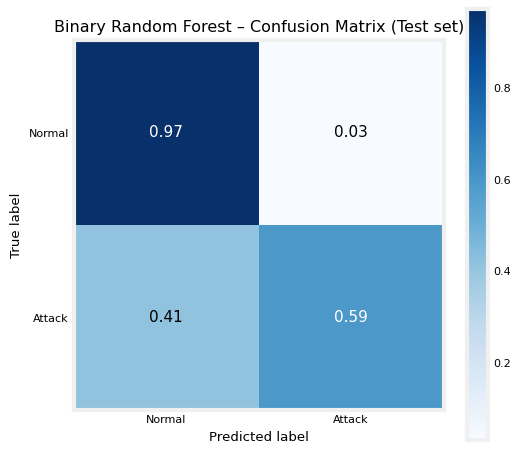
\includegraphics[width=0.7\textwidth]{conf_bin.png}
    \caption{Normalized confusion matrix for binary Logistic Regression}
    \label{fig:binary_lr_cm}
\end{figure}
\FloatBarrier

In addition to the fixed train/validation/test evaluation, stratified 5-fold cross-validation is performed for the binary Logistic Regression baseline. Across folds, the model achieves a mean accuracy of $0.954 \pm 0.001$ and a mean macro-averaged F1-score of $0.950 \pm 0.001$, indicating stable performance across different training subsets under class imbalance.

\subsection{Random Forest}
The Random Forest classifier is evaluated using a reduced feature representation consisting of the top-20 features selected via Random Forest feature-importance scores, as described in Section \ref{sec:models}. This feature subset is used consistently across both binary and multi-class Random Forest experiments. On the binary test set, Random Forest achieves an accuracy of 0.752 and a macro-averaged F1-score of 0.750. Recall is 0.972 for normal traffic and 0.585 for attack traffic. The ROC--AUC on the test set is 0.962. Figure \ref{fig:binary_rf_cm} presents the normalized confusion matrix for the binary Random Forest classifier on the test set.
\begin{figure}[htbp]
    \centering
    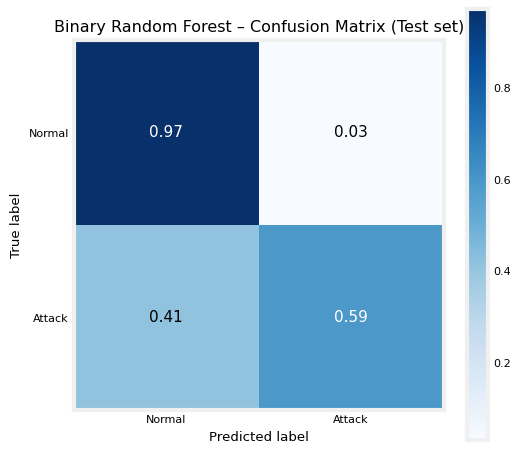
\includegraphics[width=0.7\textwidth]{conf_bin.png} 
    \caption{Normalized confusion matrix for binary Random Forest}
    \label{fig:binary_rf_cm}
\end{figure}
\FloatBarrier

\subsection{Neural Networks}
Although neural networks are not always necessary or consistently superior to classical machine-learning techniques on intrusion-detection datasets, their ability to learn higher-order feature interactions makes them a valuable comparison point. Neural networks are therefore introduced as a third modeling family to assess whether their greater representational capacity provides advantages beyond linear and tree-based methods. On the binary test set, the Neural Network achieves an accuracy of 0.778 and a macro-averaged F1-score of 0.780, with a ROC--AUC of 0.940. Class-specific recall is 0.925 for normal traffic and 0.675 for attack traffic. Figure \ref{fig:binary_nn_cm} shows the normalized confusion matrix for the binary Neural Network on the test set.
\begin{figure}[htbp]
    \centering
    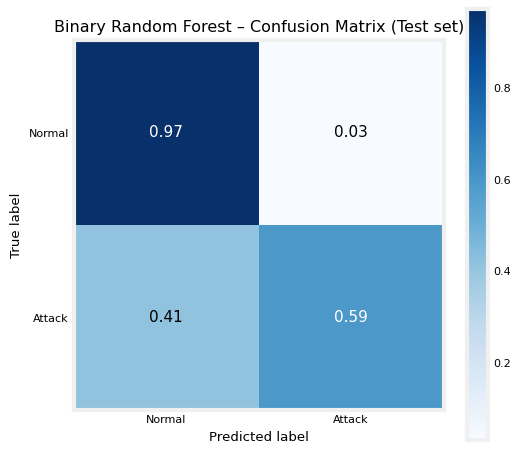
\includegraphics[width=0.7\textwidth]{conf_bin.png}
    \caption{Normalized confusion matrix for binary Neural Network}
    \label{fig:binary_nn_cm}
\end{figure}
\FloatBarrier
\vspace{-1.5em}

\section{Multi-class Classification Results}

In the multi-class setting, models are required to distinguish between normal traffic and four specific attack categories: DoS, Probe, R2L, and U2R. Table \ref{tab:multiclass_results} summarizes the performance of the three models across these categories on the test set.
\begin{table}[htbp]
\centering
\caption{Multi-class classification performance (Recall per class) on the test set.}
\label{tab:multiclass_results}
\begin{tabular}{lccccc}
\toprule
Model & Normal & DoS & Probe & R2L & U2R \\
\midrule
Logistic Regression & 0.934 & 0.811 & 0.655 & 0.046 & 0.160 \\
Random Forest       & 0.972 & 0.793 & 0.748 & 0.044 & 0.010 \\
Neural Network      & 0.925 & 0.776 & 0.702 & 0.165 & 0.700 \\
\bottomrule
\end{tabular}
\end{table}

The results highlight significant differences in how model families handle class imbalance. While Random Forest achieves the highest recall for the majority classes (Normal and Probe), it struggles significantly with the rarest categories, R2L and U2R. In contrast, the Neural Network (specifically Model 3MCv3 with class weighting) demonstrates superior sensitivity to these critical minority attacks, achieving a U2R recall of 0.700, albeit at a slight cost to overall accuracy. Figure \ref{fig:multi_rf_cm} and Figure \ref{fig:multi_nn_cm} present the non-normalized confusion matrices for the Random Forest and Neural Network multi-class models, respectively. These matrices illustrate the absolute error patterns and the models' ability to correctly categorize specific attack types.
\begin{figure}[htbp]
    \centering
    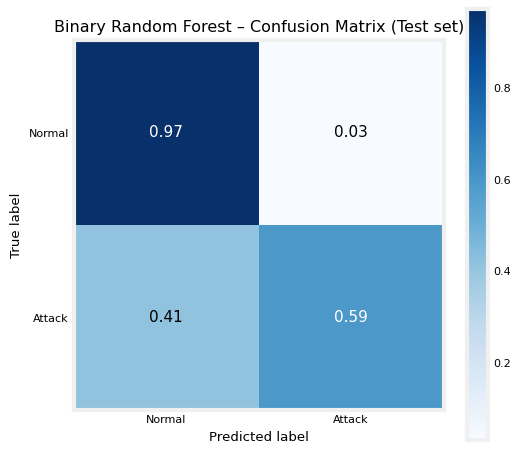
\includegraphics[width=0.7\textwidth]{conf_bin.png}
    \caption{Confusion matrix for multi-class Random Forest}
    \label{fig:multi_rf_cm}
\end{figure}
\FloatBarrier
\vspace{-1.5em}
\begin{figure}[htbp]
    \centering
    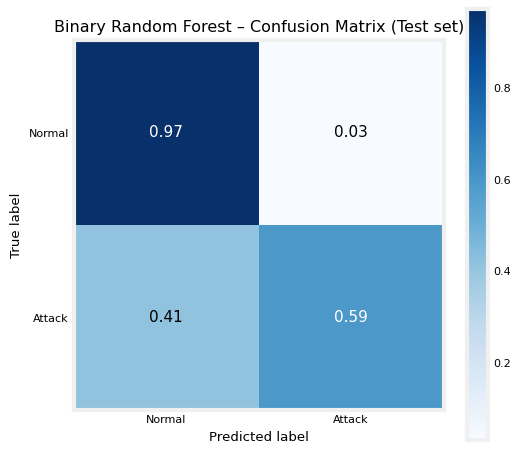
\includegraphics[width=0.7\textwidth]{conf_bin.png}
    \caption{Confusion matrix for multi-class Neural Network}
    \label{fig:multi_nn_cm}
\end{figure}
\FloatBarrier
\vspace{-1.5em}

Overall, the transition from validation to test sets reveals a consistent performance drop across all models, confirming that the NSL-KDD test set contains unseen attack variations that challenge the generalization capabilities of the trained classifiers.
% ... and so on until
\chapter{Discussion}
\label{cha:n}
\section{Interpretation of Findings}
This project compared Logistic Regression, Random Forest, and Neural Network models for intrusion detection on the NSL-KDD dataset using both binary and multi-class classification. While detailed performance metrics are reported only for the held-out test set, an important observation across all models is the substantial drop in performance from validation to test data, indicating limited generalization to unseen traffic patterns. Across all models, performance on the official NSL-KDD test set is notably lower than on the validation split, indicating limited generalization to unseen traffic patterns. This gap is expected, as the test set deliberately includes attack types and distributions that are under-represented or absent during training. Higher-capacity models, particularly Random Forest and Neural Networks, exhibit a larger relative drop in performance, suggesting that strong validation results do not necessarily translate into robust test-set performance.

In the binary intrusion-detection task, all models achieve high overall accuracy and favorable ROC characteristics on the test set. However, from a security perspective, false negatives, attacks that are incorrectly classified as normal traffic, represent the most critical failure mode, as they correspond to undetected intrusions. Analysis of the confusion matrices and class-specific recall shows that Logistic Regression produces the highest number of false negatives among the evaluated models, reflecting a conservative decision boundary that prioritizes correct classification of normal traffic. Random Forest reduces the number of false negatives relative to Logistic Regression but still misclassifies a non-negligible fraction of attacks as normal, despite strong ROC--AUC values. The Neural Network achieves the lowest false-negative rate and the highest recall for attack traffic on the test set, indicating superior sensitivity to malicious behavior. These findings illustrate that ROC curves alone are insufficient for evaluating intrusion-detection performance, as they summarize ranking ability rather than actual operational decisions. Metrics that directly reflect missed attacks, such as recall for the attack class and the absolute number of false negatives, provide a more meaningful assessment of security effectiveness.

The generalization challenge becomes substantially more severe in the multi-class setting, where the task shifts from distinguishing normal from malicious traffic to discriminating between highly imbalanced attack categories. This setting exposes significantly larger differences between models, particularly when evaluation emphasizes attack sensitivity rather than class frequency. When the Normal class is excluded from metric averaging, attack-only macro recall drops substantially relative to standard macro recall for all models, demonstrating that apparent performance on the multi-class task is largely driven by correct classification of dominant classes rather than reliable attack-type detection.

Logistic Regression achieves the highest attack-only macro recall among the evaluated models. However, this result reflects a tendency toward over-generalization rather than precise attack discrimination. While recall reaches approximately $0.45$ for R2L and $0.57$ for U2R, these gains are accompanied by very low precision, indicating that the model frequently assigns minority attack labels to non-rare samples. This behavior is consistent with the limitations of linear decision boundaries in a feature space where rare attacks overlap substantially with normal traffic, leading to increased false positives as the model attempts to compensate for class imbalance. In contrast, Random Forest exhibits the weakest performance on attack categories despite its strong results in the binary setting. Recall for R2L ($\approx 0.002$) and U2R ($\approx 0.030$) is near zero, indicating that these attacks are almost entirely misclassified as normal traffic. The confusion matrices confirm that Random Forest prioritizes stable separation of dominant patterns while effectively ignoring minority attack signatures. This outcome can be attributed to both extreme class imbalance and feature importance-based learning, which favors attributes for frequent classes and suppresses weak but security-critical signals associated with rare attacks.

The Neural Network provides the most balanced multi-class attack detection. Although recall for R2L remains modest, detection of U2R improves substantially ($\approx 0.70$), demonstrating that higher-capacity models can exploit subtle feature interactions that are inaccessible to linear or tree-based approaches. However, this improvement is accompanied by increased confusion among non-dominant classes, reflecting unstable decision boundaries in regions of the feature space with limited training data. This trade-off explains why macro-averaged $F_{1}$-scores remain considerably lower than weighted metrics, despite improvements in minority recall.

Overall, these findings indicate that multi-class intrusion detection on NSL-KDD is constrained less by model choice than by data characteristics. Aggregate metrics obscure critical weaknesses in attack detection, while class-sensitive measures reveal that rare attacks remain difficult to identify. The results suggest that future improvements are more likely to arise from data-centric strategies, such as hierarchical detection pipelines, targeted resampling, or anomaly-based modeling, than from increased model complexity alone.

In the binary neural network setting, the default decision threshold of $0.5$ was not assumed a priori. Instead, decision thresholds were analyzed using validation-set precision--recall characteristics, and the threshold yielding the best macro-averaged $F_{1}$-score on the validation set was selected for final evaluation. With the changed decision threshold, both models achieve a better accuracy for recalling attacks.

\section{Contextualize with Literature}

The results obtained in this study are consistent with established findings in the NSL-KDD literature, while also exposing limitations that are frequently masked by aggregate performance metrics. Prior benchmark studies consistently report very high overall accuracy for tree-based models. For instance, Abrar et al. demonstrate that Random Forest, Extra Trees, and Decision Tree classifiers achieve accuracies exceeding 99\% on the NSL-KDD dataset when evaluated primarily using global accuracy and class-frequency weighted metrics \cite{abrar2020machine}. Similar conclusions are reported by Hegde et al. and Hong et al., who identify Random Forest as the strongest performer across accuracy, precision, and ROC--AUC after preprocessing and feature selection \cite{hegde2024intrusion, hong2021machine}. Our binary classification results align closely with these findings: all evaluated models achieve high accuracy and $F_{1}$-scores, confirming that ML-based IDS can effectively separate normal from attack traffic under the NSL-KDD benchmark.

In contrast, when extending the analysis to the multi-class setting and emphasizing attack-centric metrics, our results diverge from much of the prior literature. While many earlier studies report macro-averaged metrics that include the dominant normal and DoS classes, our use of attack-only macro recall reveals substantially weaker performance on rare attack categories such as R2L and U2R. This outcome is consistent with the foundational analysis by Tavallaee et al., who highlight that NSL-KDD, despite improvements over KDD’99, remains highly imbalanced and that minority attack types are inherently difficult to model reliably \cite{tavallaee2009detailed}. In our experiments, Random Forest exhibits near-zero recall for R2L despite strong overall accuracy, whereas Logistic Regression attains higher recall for rare classes at the cost of severe over-generalization and very low precision. Neural Networks provide a more balanced compromise, improving minority-class recall while increasing confusion among non-dominant attack categories.

These differences can be attributed primarily to methodological choices. Many reference studies prioritize accuracy-driven model selection, employ aggressive feature selection, or rely on ensemble configurations that implicitly favor majority classes. In contrast, our evaluation explicitly isolates attack detection performance and assesses generalization to rare attacks using attack-focused metrics. As a result, this work complements existing research by demonstrating that high headline accuracy does not necessarily imply effective intrusion detection for infrequent but security-critical attack types. The key contribution of this project therefore lies not in exceeding reported accuracy levels, but in providing a more nuanced, attack-aware assessment of IDS performance. This finding is consistent with earlier critiques showing that aggregate accuracy can mask poor detection of rare and previously unseen attack types under class imbalance \cite{tavallaee2009detailed}.

\section{Limitations and Future Work}

Despite the strong overall performance achieved by the evaluated models, several limitations limit the conclusions of this study. First, the NSL-KDD dataset remains highly imbalanced, with rare attack categories such as R2L and U2R representing only a small fraction of the data. This imbalance leads to substantial class overlap in the feature space and severely limits the ability of all evaluated models to detect minority attacks in the multi-class setting. Second, the fixed feature representation restricts discrimination between rare attacks and normal traffic, as many security-critical signals are weak and easily overshadowed by dominant patterns. Third, evaluation is limited to a single benchmark dataset. While NSL-KDD enables controlled comparison, it does not fully capture the diversity and dynamics of modern network traffic.

Future work should therefore prioritize data-focused strategies rather than increased model complexity. Feature selection techniques aimed at reducing class overlap, such as class-conditional importance ranking or embedded selection methods, could help isolate discriminative attributes for rare attacks. Hierarchical detection architectures are another promising direction. A staged pipeline could first separate normal from attack traffic, then classify broad attack categories, and finally identify specific subtypes. This approach can reduce the difficulty of direct multi-class learning under severe class imbalance. Finally, cost-sensitive or anomaly-aware learning methods could be applied. Weighted loss functions or hybrid anomaly--classification models can explicitly penalize missed U2R and R2L attacks and improve recall on these critical classes. These approaches directly address the main limitations of this study and would support more practical intrusion detection deployment.

\section{Updates based on the poster presentation feedbacks}

Following the feedback received during the poster presentation, several refinements were integrated into the study to enhance the depth and clarity of the analysis. A significant methodological update involved the additional use of one-hot encoding for categorical features, ensuring that the models could more effectively interpret non-numerical relationships within the data. To better illustrate the foundational challenges of the dataset, an additional graph was included to explicitly visualize the class imbalance issue, highlighting the disparity between dominant traffic and minority attack types. 

The evaluation framework was also strengthened by prioritizing security-critical metrics. Specifically, the analysis now incorporates attack-only macro recall to provide a more realistic assessment of model performance across imbalanced categories, moving beyond the optimistic bias of standard averages. Furthermore, the results section was updated to place a deliberate focus on false negatives. By analyzing these undetected intrusions more closely, the study offers a more nuanced perspective on the operational risks and the sensitivity required for effective real-world intrusion detection.
\chapter{Conclusion}
\label{cha:conclusion}
This study investigated the effectiveness of Logistic Regression, Random Forest, and Neural Network models for intrusion detection on the NSL-KDD dataset, addressing both binary and multi-class classification settings under severe class imbalance. The results show that, while all models achieve high accuracy in the binary task, performance drops substantially on the official test set, highlighting limited generalization to unseen attack patterns. In the multi-class setting, aggregate metrics hide important weaknesses in rare attack detection, highlighting the need for attack-focused evaluation. Logistic Regression over-generalizes, Random Forest favors dominant patterns, and Neural Networks improve minority recall but introduce higher complexity and class confusion. Overall, Random Forest provides the most balanced trade-off between performance, interpretability, computational efficiency, and stability, despite its limited effectiveness on rare attack detection. The primary insight of this work is that model choice alone is insufficient to address multi-class intrusion detection challenges. Future progress will depend on improved data representations, class-aware evaluation, and validation under more realistic conditions.


% The bibliography comes after the appendices.
% You can replace the standard "abbrv" bibliography style by another one.
\bibliographystyle{ieeetr}
\bibliography{references}

\end{document}
